In this section, we empirically evaluate Sparta's performance in a series of experiments on six benchmarks, ranging from image recognition, natural language processing to random forest and time series prediction. We implemented applications based on Tensorflow and executed through Sparta's actuator interface.  In each experiment, Sparta takes inputs of task program, workload dataset and threshold temperature. There are two goals of scheduling by Sparta: the first is to limit the CPU temperature under the threshold; secondly, Sparta accelerates the task to the fullest extent without overheating the edge cloud devices.

\subsection{Machine Learning Benchmarks}

To comprehensively evaluate the efficacy and efficiency of Sparta, we implemented 6 machine learning benchmarks, which consist of four categories: image recognition, natural language processing, ensemble learning and time series analysis. We aim to test Sparta on a variety of machine learning applications that represent different execution patterns.

\subsubsection{WTB\_Train}

is the first image recognition application that we use as a benchmark trains a convolutional neural network (CNN)~\cite{ref:cnn} on the top of ResNet50~\cite{ref:resnet}. The training dataset contains animal images from a wildlife monitoring system called "Where's The Bear" (WTB)~\cite{ref:wtb}. "Where's The Bear" is an end-to-end distributed data acquisition and analytical system that automatically analyzes camera trap images collected by cameras sited at the Sedgwick Natural Reserve~\cite{ref:sedgwick} in Santa Barbara County, California. In total, there are five classes that we consider: Bear, Coyote, Deer, Bird and Empty, by which we label images for training tasks. We also up-sampled minority classes using the Keras Image Data Generator~\cite{ref:datagen}, since the class size is unbalanced due to the frequency of animal occurrences. Doing so ensures that the classification model is not biased. We resized every image in the dataset to $1920 \times 1080$, and for each class, the dataset contains 251 images used to train the CNN model. Once the training is complete, the application stores this model in hdf5 format in object storage. 

The WTB\_Train application has a cold start at the beginning of the execution, since it loads a neural network model and a large dataset. Once it completes loading, the entire training process has relatively consistent CPU usage and temperature. 

\subsubsection{WTB\_Inf}

Based on WTB\_Train, we inference the type of wildlife in camera trap pictures by the second application. It loads the trained model from WTB\_Train and, for each picture, it assigns probabilities to five classes we consider in the training dataset by Softmax function. In terms of the execution pattern, WTB\_Inf runs in short bursts compared to WTB\_Train. Therefore, the CPU usage and temperature fluctuate dramatically throughout the execution of this benchmark.

\subsubsection{MNIST}

 is a dataset containing grayscale pictures of handwritten digits, in which it has 60,000 examples as training set and 10,000 examples as testing set. Based on the dataset, we train a 2-layer convolutional neural network~\cite{ref:MNIST} and test its accuracy in the third application. In contrast to WTB benchmarks, the size of pictures is smaller ($28 \times 28$) and the model is simplified in MNIST. We aim to evaluate Sparta on an application that includes both training and inference process. 

\subsubsection{BiLSTM} is a sentiment analysis application based on a dataset of the Internet Movie Database (IMDB) movie reviews. It consists of 25,000 sequences each for training and testing. The model is constructed as a bidirectional LSTM with a classification layer using sigmoid activation function. We train the model by the training dataset and validate by testing dataset in BiLSTM application. Since it has a large dataset and a complex model, the execution pattern is long-running and consistent in CPU usage and temperature.


\subsubsection{Decision\_Forest} is an implementation of deep neural decision forests~\cite{ref:decision_forest} that classifies high-earning individuals from the pool. The benchmark leverages the United States Census Income Dataset~\cite{ref:uci} that has 48,843 instances with 14 features, including age, education, occupation, etc. The dataset is split up that the training part has 32,561 instances and the testing part has 16,282 instances. The application has three phases: it firstly processes the dataset by encoding input features. Then, it trains a deep neural decision tree model. Based on that, the application trains a neural decision forest model consists of a set of neural decision trees. Therefore, the usage and temperature of CPU increasingly grows throughout the process.


\subsubsection{Time\_Series} is a time series prediction application built on the climate data recorded by the Max Planck Institute for Biogeochemistry~\cite{ref:jena}. The dataset has 14 features such as temperature, pressure, humidity, etc. and the sampling frequency is 10 minutes. The time frame of the dataset ranges from Jan. 10th, 2009 to Dec. 31st, 2016. The application uses 300,693 rows to train a single-layer LSTM model, by which we can predict temperature in next 72 timestamps (12 hours) given the temperature in the past 720 timestamps (120 hours). We intend to evaluate Sparta on an application with light model and large dataset.

% Execution pattern table

\subsection{Experimental Setup}

The edge cloud device we set up for experiments is Intel NUC~\cite{ref:nuc} (6i7KYK) with two Intel Core i7-6770HQ 4-core processors (6M Cache, 2.60 GHz) and 32GB of DDR4-2133+ RAM connected via two channels.  

To simulate the natural temperature in Sedgwick natural reserve, we create three thermal environments in an isolated cooler that represent cold, neutral and hot ambient temperature. In the cold scenario, the ambient temperature is 2.6\degree C and the CPU of NUC runs under 40\degree C in idle status. In the neutral scenario, the CPU of NUC starts at 51\degree C under the ambient temperature of 23.9\degree C. The hot scenario increases the ambient and CPU temperature to 43.8\degree C and 68\degree C respectively.

\begin{figure}
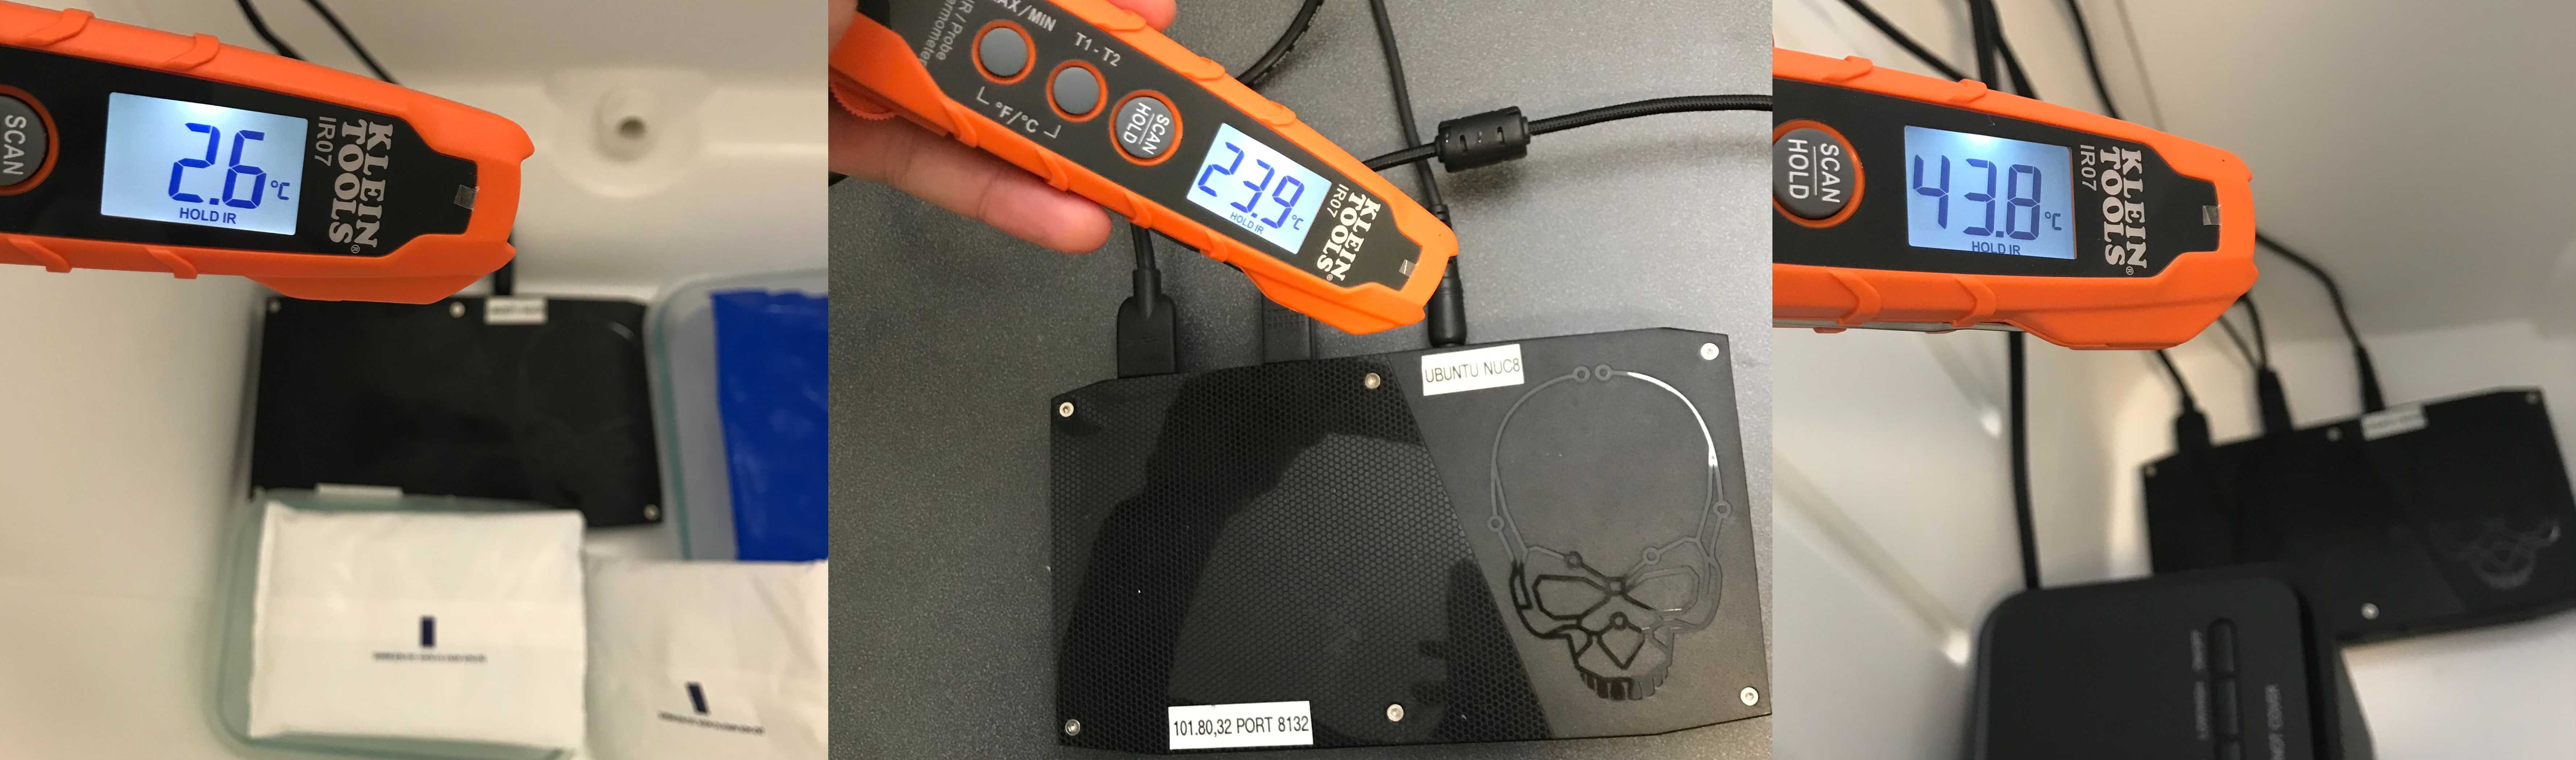
\includegraphics[width=\textwidth]{figures/thermal.jpg}
\caption{Three thermal environments in the experiment} \label{cold}
\end{figure}

\subsection{}
 